% Set the author and title of the compiled pdf
\hypersetup{
	pdftitle = {\Title},
	pdfauthor = {\Author}
}

% Like a quote but without the indent
\newenvironment{fancyquote}{
	\list{}{
		\leftmargin=0.3in
		\rightmargin=0.3in
	}
		\item[]
	{\endlist}
}

\setcounter{page}{1}

\section*{Introduction}

Unlike many of the courses, the university supplied notes for this course are of
a very high quality. This is especially true of the notes covering the first
half of the course (weeks one through six). In light of this, I've decided not
to write notes on the first half, but concentrate solely on the second half of
the course. However, it is likely that I will produce other resources such as
summary notes or flashcards for the whole of the course.

\section{The three box model}

The three box model describes the classic model of a computer. The three boxes
consist of the CPU, the memory and I/O.

\begin{figure}[ht!]
	\centering
	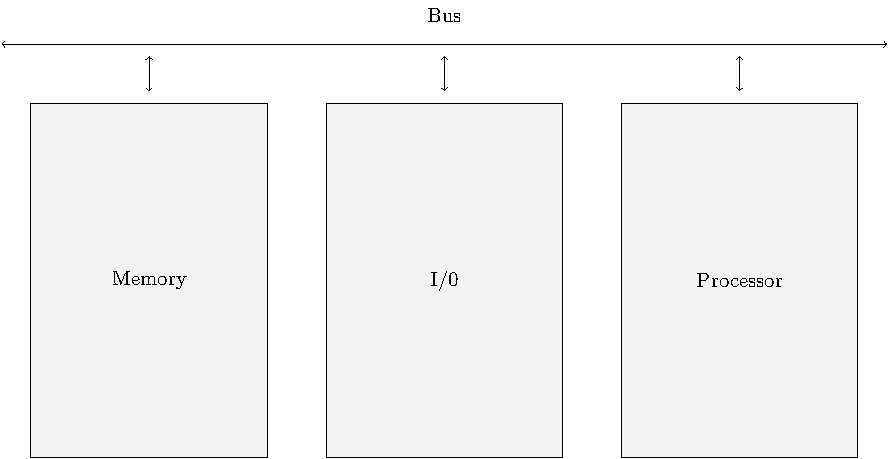
\includegraphics[width=\textwidth]{three_box_model.pdf}
	\caption{An example of the three box model}
	\label{overflow}
\end{figure}

% Take a look at the 3_box_model_description branch for info I took out from
% here

\subsection{The Amdahl/Case rule}

A computer that has one disproportionately powerful component is very wasteful
since the other components will act as a limiting factor with regard to the
speed of the computer. It's no good having a fantastically fast processor with a
tiny amount of RAM.

The Amdahl/Case rule gives us guidelines that we can use to determine sensible
specifications for components within a computer. Though there are many different
versions of this rule, it is something along the lines of:

\marginpar{MIPS stands for million instructions per second}

\begin{fancyquote}
		A balanced computer system needs about one megabyte of main memory and
		about one megabit per second of I/O per MIPS of CPU performance.
\end{fancyquote}

\subsection{CPU}

\subsubsection{The fetch, decode, execute cycle}

The CPU is essentially a large FSM\marginpar{FSM = Finite State Machine} that
loops over three operations; fetch, decode and execute in order to perform the
instructions defined in a program.

\paragraph{Fetch}\mbox{}

The processor first reads a word \marginpar{1 word = 4 bytes}from an address
that is pointed to in memory by a {\it pointer}. After the instruction has been
read, the pointer is moved on to the next address in memory.

\paragraph{Decode}\mbox{}

The instructions that are to be loaded from memory are really just a really long
list of numbers. However, each number is coded in such a way that it represents
an action. A rudimentary way of encoding such a system would be to let the
number $1$ mean 'shift bits left' and the number $2$ mean 'shift bits right'. An
operation code is obtained from the instruction and the control signals specific
to that code are then set for the FSM.

\paragraph{Execute}\mbox{}

\marginpar{A datapath is a collection of logic units to perform arithmetic or
other functions. See course supplied notes for more information on datapaths.}

In this phase, the data is moved through the datapath and the instruction that
was in memory is now performed. The processor then starts the cycle again, by
fetching an instruction from memory.

\subsubsection{Maintaining state}

A CPU is required to maintain some form of state while processing instructions,
since most instructions have interactions between one another. In order to keep
track of what's going on in between instructions, the CPU uses both the registers
that is has built in and the main memory.

It is important to realise that the whole system changes state at the same time,
driven by a central {\it clock}. This means that all the parts of the system are
in sync with each other. In fact, we can treat the system as a whole (including
the memory and registers) as a finite state machine.

\subsubsection{Address spaces}

An address space is a number of memory locations that a system can address. Each
location in memory has a unique address, which is a number.

Memory addresses are countable, i.e. you can increment one to get the next one
and decrement one to get the previous one. However, they are sometimes not
countable in the traditional sense. First of all, they are usually counted in
hexadecimal in order to save characters and enable easy conversion to binary,
with each digit converting to four bits. Second of all, the length of the word
defines the gap between each countable memory location.

\marginpar{N.b. Most processors offer the capability to address bytes in between
the words too}

For example, in 32 bit processors, words are defined as 32 bits long.
Henceforth, each memory location is contains 32 bits, and so the addresses go up
in fours. In a 64 bit processor, the gap between adjacent addressable words in
memory would be eight addresses.

The number of bits in a word is very important for a number of reasons. Longer
words usually mean longer instructions, so more information can fit inside,
meaning less instructions need to be executed to perform tasks. Also, longer
words means more addressable memory locations; in a 32 bit system, there are
$2^{32}$ memory locations, but in a 64 bit system, there are $2^{64}$
addressable memory locations. This is why 32 bit systems are limited to 4GB or
RAM.

\subsection{Memory}

Memory allows the processor to write store and load data. It is often referred
to as Random Access Memory. As opposed to hard drives, where in order to access
different locations a physical component must be moved, RAM is able to access
any location in any order with no time penalty, hence the usage of the term {\it
random}.

We can work out how many bits are required to address a memory of a given size.
In order to do this, we must find the power of 2 equal to or above the size of
the memory (in bytes), and split it into common factors (which should also be
powers of two) then we add up the powers, which will give us our number of bits.
Here are some examples:

{\bf Find the number of bits required to address 1 Kbyte of memory}

\begin{enumerate}
	\item Find the powers of two that will go into 1 Kbyte:
			1 Kybte = $2^{10}$ bytes
\end{enumerate}

{\bf Find the number of bits required to address 64M bytes of memory}

\begin{enumerate}
	\item Find the powers of two that will go into 64 Mbytes:
			64 Mybtes = $2^{26}$ bytes = $2^6 + 2^{20}$ bytes
	\item Add the powers together:
			$6 + 20 = 26$ bits
\end{enumerate}


{\bf Find the amount of memory that can be addressed by 19 bits}

\begin{enumerate}
	\item $2^{19} = 2^{10} \times 2^{9} = 1,024 \times 512 = $ 512 Kbytes
\end{enumerate}

\subsubsection{Memory caching}

A commonly used optimisation for memory is to use a cache. This is a small
amount of extra memory that is very fast to access. The values stored in memory
addresses that are being accessed frequently can be temporarily stored here
instead to avoid the comparatively slow referencing of the main memory.

\subsection{Input/Output}

IO is concerned with interfacing with peripheral devices such as keyboards,
monitors, networks etc. Each device will have an interface to a specific bus
that can communicate with memory and the CPU.

A {\it port} is a form of I/O  that is usually mapped to an area of memory. In
the eyes of the CPU, a simple output port is just an area of memory to be read
from and written to, however, it will also be mapped to some external connection
such as lights, motor or even more complicated devices such as a printer.

An input port will also 'look' like an area of memory to the CPU, however, that
area of memory will be connected to external signals.

\marginpar{Most ports are 8-bits wide, even in processors that use larger word
lengths.}

It is also possible to have bidirectional ports, however, this requires extra
coordination to ensure that reading and writing doesn't take place at the same
time.

\paragraph{Types of ports}\mbox{}

There are two main types of ports, serial and parallel. Parallel ports are as
described above; just a collection of wires that can be in the states 1 or 0. In
order to send a 1 Mbyte file over a parallel port, could either have eight
million wires or you can use only eight wires and splitting the file into one
million parts.

Serial ports only deal with single bits, and so require one wire. This may seem
very slow, but a lot of time is often spent optimising the transfer so its
speeds are comparable with parallel ports. However, serial ports often need
extra registers to signal other information such as transfer speed and the
direction of transfer.

\subsection{Buses}

A bus is a collection of signals that act together.

There are three buses used by the CPU:

\begin{itemize}
	\item {\bf Address bus}
		This is an output for the processor, and is used to specify the location
		in Memory or I/O for data to be transferred. It is usually as wide as
		the word length of the processor.
	
	\item {\bf Data bus}
		This is usually a bidirectional bus, usually as wide as a processor's
		registers (that in turn are usually as wide as a word). However, a
		smaller data bus will reduce the cost of the processor, but a larger bus
		will enable a higher bandwidth, which could let the processor fetch more
		than one instruction in one cycle!\marginpar{N.b. Another way to make a
		bus go faster is to increase the clock speed it is running at.}

	\item {\bf Control bus}
		The main function of the control bus is to specify the direction of the
		flow of data. However, it also has a lot of other functions which aren't
		relevant here.
\end{itemize}

\section{Processor design - the MU0}

The MU0 is a very simple design of processor. So simple in fact, that it can be
described within the scope of these notes. However, despite it's simplicity, it
is a complete processor and is capable of running complete programs.
% TODO: Check this
\marginpar{Since there are 4 bits for the operation inside an MU0 instruction,
we have a capacity for $2^4$ (16) different operations. Since the address space
is comprised of 12 bits, the maximum amount of addressable memory locations is
$2^{12}$, which is equal to 4096 16 bit words, making for a total of 8 Kbytes of
RAM.}

The MU0 is a 16 bit machine, that has a 12-bit address space. Instructions are
coded like so for the MU0:

\begin{figure}[ht!]
	\centering
	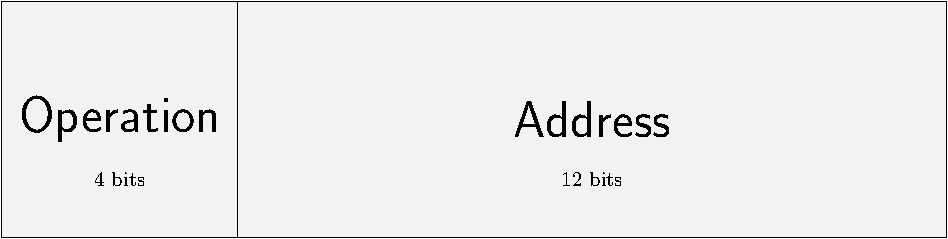
\includegraphics[width=90mm]{instruction_format.pdf}
	\caption{A sample MU0 instruction}
	\label{overflow}
\end{figure}

\subsection{The MU0 instruction set}

Since the instructions are 16 bits wide, the memory and internal data paths
inside the MU0 are also 16 bits wide. There are two registers available to
programmers (though more will be used internally).

Each instruction can have either one or zero operands. Instructions that use
more than one operand must implicitly use a register. Here is a table describing
the instruction set:

\marginpar{You might notice that there are only eight operations here even
though we have space for sixteen. The unmapped op codes are blank at the
moment, but could be used to expand the capabilities of the processor.}

\begin{center}
	\begin{tabular}{|c|c|c|}
		\hline
		{\bf Op Code} & {\bf Mnemonic} & {\bf Description}\\ \hline
		0 & LDA $[op]$ & $[op] \rightarrow Acc$\\ \hline
		1 & STO $[op]$ & $Acc \rightarrow [op]$\\ \hline
		2 & ADD $[op]$ & $Acc = Acc + [op]$\\ \hline
		3 & SUB $[op]$ & $Acc = Acc - [op]$\\ \hline
		4 & JMP $[op]$ & $PC = S$\\ \hline
		5 & JGE $[op]$ & If $Acc >= 0$ then $PC = S$\\ \hline
		6 & JNE $[op]$ & If $Acc \not= 0$ then $PC = S$\\ \hline
		7 & STP & Stop\\ \hline
	\end{tabular}
\end{center}

\subsection{Executing instructions}

Like any CPU, the MU0 goes through the fetch execute cycle for every instruction
it executes. However, since the MU0 is so simple, we can break the cycle into
more steps:

\begin{enumerate}

	\item Fetch the instruction from the memory address specified by the PC.

	\item Increment the PC

	\item Decode the instruction (i.e. read the first four bits)

	\item Get the operand for the instruction from:
		\begin{itemize}
			\item Memory for load or arithmetic instructions
			\item The instruction register for jump instructions. We look inside
			the instruction register since it is where the instruction is held
			while being decoded. The address of the operand will be encoded in
			the instruction itself.
			\item The accumulator register for store or arithmetic instructions.
		\end{itemize}

	\item Perform the operation

	\item Write the result to the PC, accumulator or memory.
\end{enumerate}

\subsubsection{The program counter}

The PC (Program Counter) is a register that contains the memory address of the
next instruction to be executed. Every time an instruction is executed, the
program counter is incremented by one.

\subsection{The MU0 datapath}

Instructions can be executed in two clock cycles of the MU0. The first cycle is
used to fetch the instruction into the instruction register, and the second is
used to decode the instruction, read the operand and store the result wherever
it needs to be stored. Please refer to the course supplied notes for the full
datapath design of the MU0.

\subsection{Registers in the MU0}

The MU0 contains three registers; ACC (Accumulator), PC (Program Counter) and IR
(Instruction Register). Only the first two are visible to the programmer (since
the job of the instruction register is to store the next instruction to be
executed after a fetch has occurred).

Each register is comprised of 16 D-type flip flops and is therefore made up of
sixteen bits. All of the flip flops are connected to the system clock, and are
therefore synchronous in their operation.

The CE (Clock Enable) signal initiates the loading of information into the
registers. If CE is high, then each flip flop will assume the input value that
it is given when the system is clocked.\marginpar{N.b. if there isn't a clock
pulse when the CE is high, then nothing will happen, since the registers only
change on each clock pulse.}

The outputs of the three registers can be def into a shared bus. Only one
register can feed into the bus at a time, and in order to coordinate this, the
OE (Output Enable) signal must be high for a register to drive the output bus.

\subsection{Register banks}

In modern processors, there are usually far more registers than in the MU0, for
example, ARM uses 16 registers and MIPS uses 32. Each register can be connected
to any port at any time. It is common to be able to perform several read/write
operations on registers in one instruction.

Like memory, registers need to be addressed using a series of bits. With 16
registers, $2^{4}$ bits are needed to address all the registers. In the MU0, we
don't need to bother with this, since it has only one programmer accessible
register, the accumulator, and $2^0=1$.

\subsection{The ALU}

The MU0 doesn't really contain an ALU (Arithmetic Logic Unit), since the ALU
contained within the MU0 doesn't have functions for logical operations such as
{\tt NOT}, {\tt AND} and {\tt XOR}. Thus it would be more accurate to simply
call the ALU inside the MU0 an Arithmetic Unit!

A typical ALU will usually contain two input buses (lets say called {\tt A} and
{\tt B}) and an output bus (called {\tt Z} in our example). The ALU in the MU0 is
capable of doing the following operations:

\begin{center}
	\begin{tabular}{|l|l|}
		\hline
		{\bf Instruction} & {\bf Description}\\ \hline
		{\tt ADD} & {\tt Z = A + B}\\ \hline
		{\tt SUB} & {\tt Z = A - B}\\ \hline
		Fetch instruction & {\tt PC = PC + 1}\\ \hline
		{\tt LDA} & {\tt Z = A}\\ \hline
	\end{tabular}
\end{center}

It is important to note that each of these operations can be expressed as an
addition:

\begin{itemize}
	\item Z = X + Y
	\item Z = X + (-Y)
	\item Z = X + 1
	\item Z = 0 + Y
\end{itemize}

This makes the implementation of the ALU easier.

Because all the MU0 ALU really does is add stuff together, its main component is
an adder. Since the MU0 is a 16 bit machine, the adder must be 16 bits too. The
most simple adder we can use for the MU0 is a 16 bit ripple-carry adder.

\subsubsection{Critical paths}

We can determine how fast a circuit can run by finding the critical path of the
circuit. The critical path is defined as the path some logic can take from one
end of the circuit to the other that will take the most time. If we are given
the time it takes for each gate used in the circuit to change state, then we can
simply add up all the times in each path, and see which one is longest.

When we have the time it takes to execute the critical path, we can use the
formula $f = \frac{1}{T}$ to find the maximum clock frequency of the circuit

\subsubsection{The structure of the ALU in the MU0}

Though the ALU inside the MU0 is mostly comprised of just an Adder, there are a
few more things going on too. There is some preconditioning that is applied to
the input buses. For the following commands, the following preconditions are
applied:

\begin{center}
	\begin{tabular}{|c|c|c|}
		\hline
		{\bf Function} & {\bf First bus} & {\bf Second bus}\\ \hline
		{\tt ADD} & Normal & Normal\\ \hline
		{\tt SUB} & Normal & Inverted\\ \hline
		{\tt INC} & Normal & 1\\ \hline
		{\tt output = second\_bus} & 0 & Normal\\ \hline
	\end{tabular}
\end{center}

\marginpar{'1' here means '000000000000001' and '0' means '000000000000000'}


\subsubsection*{Selecting what logic to use in an ALU}

An important feature of any ALU is the ability to select what Logic to employ on
the input data. This is often accomplished by way of another bus going into the
ALU carrying the code of the logic function to execute.

It is possible to use a multiplexer to execute certain logical tasks. Setting
all bits to 0 in a bus for example could be done in verilog like so:

\begin{listing}{1}
module setzero(fun, in, out);
	output [15:0] out;
	input [15:0] in;
	input fun;

	assign out = fun ? 0 : in
endmodule
\end{listing}

The last line of the verilog block does the actual work here. It is a
conditional operator that will set the output to 0 if the {\tt fun} input is
high, and set the output to the {\tt in} bus if {\tt fun} is low.

\subsubsection{General ALU's}

In general, ALU's have many more features than the one in the MU0. Such features
may include:

\begin{itemize}
	\item Do nothing to the data (also known as {\it true data})
	\item Complement the input (invert all the bits)
	\item Zero the bits
	\item Make all the bits 1
\end{itemize}

\subsubsection{Decoding the function code in an ALU}

The required value of the control bits to activate any given function in the ALU
are arbitrary, though choosing a good set of values is desirable since it may
make the implementation easier.

\subsection{Making decisions in the ALU}

In any processor, when an {\tt if} statement is executed then the processor will
most likely (under many layers of syntax and abstraction) perform a branch.

In the MU0, the accumulator is used to evaluate conditions, however, in some
other architectures, the result of a comparison is stored in a separate {\it
condition code} register (these results are often referred to as {\it flags}).

In the MU0, there are only two conditional branches:

\begin{enumerate}
	\item Jump if {\tt Acc} is positive
	\item Jump if {\tt Acc} is not 0
\end{enumerate}

This also allows programmers to test for a specific value, since you can use
{\tt SUB} to get 0 if two values are equal and then use the second jump
condition.

\subsection{How the MU0 executes operations}

All instructions execute in the MU0 in two instruction cycles. The first cycle
involves the instruction being fetched from memory and read into the instruction
register, while the second cycle is when the instruction is decoded and
executed.

\subsubsection{Fetching an instruction}

When the processor is in the fetch state, the value at the memory address
specified by the program counter register is fetched into the instruction
register. The PC is then incremented so that the next instruction is fetched
when this one has finished executing.

\marginpar{Even if the instruction is a jump, the PC is still incremented after
the fetch. This is because the instruction hasn't been decoded while it is
being fetched so the processor has no way of knowing if it's a jump.}

\subsubsection{Executing an instruction}

When the processor starts to decode the instruction, its behaviour is defined by
the instruction that it is executing. It will first read the instruction code
and then follow one of the eight possible paths of execution depending on what
the instruction is to be executed.

The control signals that control all of the registers and the ALU depend on the
value of F. The data in the instruction is then just piped through the
processor, being mutated by the various components as it goes.

\subsubsection{Implementing an instruction decoder in verilog}

We can create a block of verilog code that will compile down to a FSM that will
translate a three bit input from the instruction into the control lines to the
various components inside the processor.

First, we need an always block to trigger whenever the {\tt state} or the
instruction register {\tt IR} changes:

\begin{listing}{1}
always @ (state, ir)
\end{listing}

After that, we need to check the state of {\tt state} to see if the processor is
loading an instruction or decoding one:

\begin{listingcont}
	if(state==0)
		// We're fetching an instruction
		begin
		// Set the control lines to fetch
		// an instruction from memory
		Asel = 0;
		...
		Ren = 1;
		Wen = 0;
		end
	else 	// The state must be equal to 1 
			// therefore we're decoding
		begin
\end{listingcont}

Now we need a case statement to decode the instruction code:

\begin{listingcont}
	case(ir[15:12])
		// LDA
		0: 	begin
			Ren = 1;
			Wen = 0;
			Asel = 0;
			Xsel = 1;
			M[1:0] = 2'b10;
			...
			end
		1:	begin
			...
			end
		...
		7:	begin
			...
			end
	endcase
end
\end{listingcont}

\subsection{Timing in the MU0}

The MU0 employs a synchronous timing design. This means that all state changes
happen at the same time, at the positive edge of the clock. This is handy, since
when the control signals begin to be calculated at the start of decoding, the IR
is latched and they have a whole cycle to settle.

In order to employ a synchronous design, we must assume that the clock signal
arrives at all the flip flops at the same time, and that there is enough time
between clock ticks so that the slowest possible set of logic changes have time
to take place.\marginpar{This would be the {\it worst case critical path}.}

In order to calculate the fastest timing we can do, we must find the critical
path of the processor (i.e. the slowest path data can take). We the have to use
the formula:

\[
	\textrm{\it Time period} = \frac{1}{frequency}
\]

to find the maximum clock frequency. So, if the critical path was $20ns$, then
the fastest clock frequency we could set would be:
\[
	\frac{1}{20\times10^{-9}} = \SI{50}{\mega\hertz}
\]

\section{Optimising an architecture}

There are three main ways that we can optimise a processor so that it can run
faster, they are:

\begin{itemize}
	
	\item Improving the technology so that there are more transistors on the
	chip. This means that it can do more logic at any one time.

	\item Shrink the critical path so that the clock speed can be increased.
	This often has to balance power consumption and heat production with
	speed.

	\item Restructure the design so that each clock cycle can do more stuff.
	An example of this may be when an instruction is both fetched; the PC
	must be read and the value must be fetched from the memory. These
	operations could be done one after another, but it would mean that the
	fetch stage of an instruction would take twice as long, and the
	processor would take 1.5 times longer to execute.

\end{itemize}

\marginpar{A metric often used here is the number of clocks per instruction
(CPI).}

\subsection{Carry look ahead}

Adders are an important and oft used component in any computer architecture.
Since there are so many of them, they are a good target for optimisation. It is
possible to work out whether the adder will generate a carry or not almost as
soon as the input bits arrive. Just by looking at the input bits, we can tell if
{\tt Cout} will be Zero, {\tt Cin} or One.

\begin{center}
	\begin{tabular}{|c c|c|}
		\hline
		{\bf A} & {\bf B} & {\bf Cout}\\ \hline
		0 & 0 & 0\\
		0 & 1 & {\tt Cin}\\
		1 & 0 & {\tt Cin}\\
		1 & 1 & 1\\
		\hline
	\end{tabular}
\end{center}

Working out the carry out and propagating it onto the next adder is a technique
called {\bf Look Ahead Carry}.

\subsection{Parallelism}

One obvious way to improve the speed of any architecture is to make two things
happen at once; i.e. make things happen in parallel. There are two different
ways of achieving parallel execution in a computer:

\begin{itemize}

	\item Start one instruction before another has finished executing (e.g. by
	decoding one instruction while fetching the next)

	\item Compute several instructions at the same time (e.g. by having two
	processing cores)

\end{itemize}

\marginpar{\vspace{-6em} Using more than one processing core, or executing 
multiple instructions in parallel is also known as superscalar processing.}

However, it is often the case that despite using parallel execution, gaining a
speed increase of twice what was observed without using parallel execution is
often not the case, since systems would be more complicated. However, the cost
of the system would usually increase by at least two times, since it would be
harder to make and would contain more components.


\subsection{Adding bitwise operators to an ALU}

If you wanted to add bitwise operators to an ALU, all you need to do is put the
respective gates before the inputs into the ALU. The specific bitwise operator
to be used can be selected by using a multiplexer.

An optimisation here, would be to recognise that it is possible to implement an
XOR gate by just disabling the carry on the adders inside the ALU.

\section{Bit shifting}

In order to multiply or divide a number by two in binary, all you have to do is
shift the numbers to the left or right by one place. This is called a bit shift.

You may notice, that when you shift to the right, data is lost. This problem can
be mitigated by doing two things:

\begin{itemize}

	\item A logical shift right (where zeros are shifted in to the MSB).

	\item An arithmetic shift right (where the existing MSB is copied to the new
	MSB). This will preserve the sign of the number if it is being interpreted
	as a signed integer.

\end{itemize}

However, since in most (if not all) computer systems, a number only has a finite
set of binary digits, shifting to the left can also result in the loss of data.
When doing a left shift, a zero is always shifted in to the right side.

\subsection{Bit rotations}

It is also possible to rotate bits, so when you do a shift, copy the bit that
would be shifted out, and insert it onto the side of the number that is gaining
a new bit. In this way, data is only never mutated, and never lost.

\subsection{Implementing a single shift}

The only components needed to implement a single place bit shift are
multiplexers. See page 47 in the notes for a diagram.

\subsection{Shift registers}

A shift register is just like a normal register, but it inputs and outputs the
data in parallel. You can also give them bits one at a time, so that all the
bits in the register are shifted along to make room for the new one and the end
bit 'falls off' and is lost.

Often, lots of extra components are required to implement a shift register, so
it's not usually worth implementing inside a processor. However, they are often
used for tasks involving I/O.

\section{Multiplication}

Simple multiplication would involve starting with a register set to {\tt 0}, and
then adding {\tt M} to the register {\tt N} times. This however, is very slow
for large numbers. \marginpar{The time complexity would be $O(nm)$.} This would
be simple to implement though, since all you really need is an adder and some
logic to count from {\tt 0} to {\tt N}.

A faster way to multiply numbers would be using long division:

\begin{enumerate}
	\item Start with zero in an accumulator
	\item Get the least significant digit of {\tt M}. We'll call this {\tt X}.
	\item Multiply {\tt N} by {\tt X}.
	\item Add the result to the accumulator.
	\item Multiply {\tt N} by 10.
	\item Make {\tt X} the next least significant digit of {\tt M}.
	\item Repeat steps 3-6 until you run out of digits in N
\end{enumerate}

Here's an example of applying the algorithm to the multiplication $453 \times
643$:

\begin{center}
	\begin{tabular}{c c c}
		{\tt Accumulator} & {\tt X} & {\tt M}\\ \hline
		00000000 & 3 & 00000643\\
		00001929 & 3 & 00000643\\
		00001929 & 5 & 00006430\\
		00034079 & 5 & 00006430\\
		00034079 & 4 & 00064300\\
		00291279 & 4 & 00064300\\
	\end{tabular}
\end{center}

Here, we're using base 10 to do our calculations, but a computer would use base
2. This is no problem, since we'd only ever have to multiply by 1 or 0 (which is
easy) or multiply by 2 (instead of 10, which is just a shift).

Here's an example in base 2. Multiply $0101$ by $0010$:

\begin{center}
	\begin{tabular}{c c c}
		{\tt Accumulator} & {\tt X} & {\tt M}\\ \hline
		0000 & 1 & 00010\\
		0010 & 1 & 00010\\
		0010 & 0 & 00100\\
		0010 & 0 & 00100\\
		0010 & 1 & 01000\\
		1010 & 1 & 01000\\
		1010 & 0 & 10000\\
		1010 & 0 & 10000\\
	\end{tabular}
\end{center}

We can check that using base 10: $5 \times 2 = 10$.

It is possible to terminate this algorithm early if the remaining bits to be
multiplied are all zeros. This is called {\bf early termination}.

%TODO: The notes explain this so badly (page 50). Can it be cleaned up?
If the multiplication goes over the number of bits available inside the number,
we can use {\bf modulo arithmetic}. This is when we will take the answer and
find the modulus of it with $2^n$ where $n$ is the number of bits in the number.

\marginpar{If we use modulo arithmetic, then multiplication will work just fine
on signed integers too!}
